\documentclass{report}
\usepackage[utf8]{inputenc}
\usepackage{graphics}
\graphicspath{ {./images/} }
\usepackage{multicol}

% width,height
\usepackage[a4paper, total={7in, 10in}]{geometry}

\title{IOT Based Smart Farming}
\author{TRISHAA S}
\date{\today}

\begin{document}

\begin{titlepage}
    \centering
     
        
\includegraphics{logo3}\\
        Computer Science and Engineering\\
        Shiv Nadar University, Chennai\\
        22 January 2023
        
        \vspace*{3cm}
        \Huge
        \textbf{IOT Based Smart Farming}
        
        \vspace*{0.6cm}
        \Large
        \textit{IOT Architechture And Protocol}
        
        \normalsize
        \vspace*{1cm}
        TRISHAA S\\
        \vspace{0.2cm}
        21011101134\\
        \vspace{0.2cm}
        AI-DS B\\
        
        \vfill
        
        %\large
        %\vspace*{0.1cm}
        Sustainable Farming Methods
        
        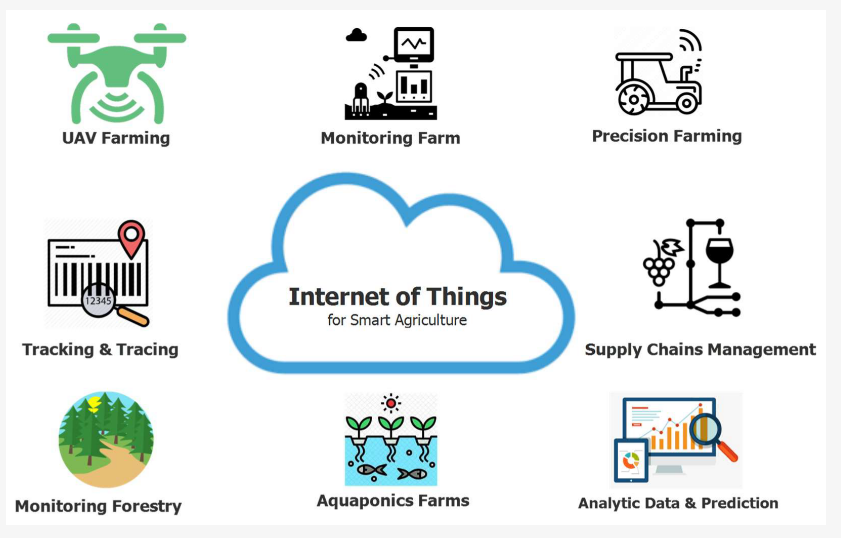
\includegraphics{Folder/images/IMG1.png}\\
        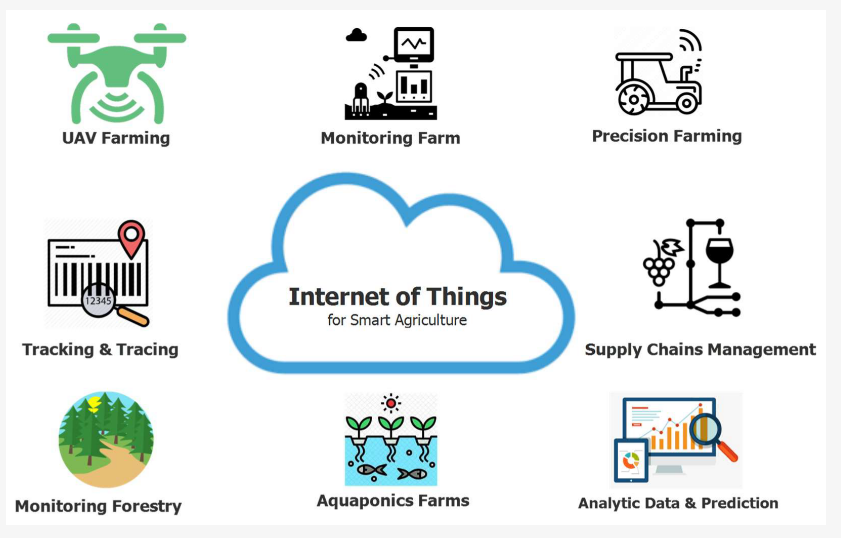
\includegraphics[scale=0.25] {Folder/images/IMG1.png}
        \vfill
        %\includegraphics[scale=0.5]{logo}
        
        
        %\vspace*{1cm}
    
\end{titlepage}

    
\begin{center}
        \section*{SMART FARMING}
\end{center}
\setlength{\columnsep}{1.0cm}
    \large
    \section*{Summary}

Internet Of Things is a revolutionary technology that 
represents the future of communication & computing. The area 
of implementation of IoT is vast and can be implemented in 
every field, One such field is namely Smart Farming. Nowadays, 
the digital transformation of the agricultural sector is 
considered a priority in order to face the numerous challenges 
presented in the fields.Smart farming systems can thus provide
farmers meaningful real time environmental data from the 
cultivation fields which will therefore boost competitiveness 
and profit.\\
\\
Traditional Farming and Smart Farming are very different from 
each other in every way. In Traditional Farming old methods 
are used where the demand for crops is not pre-assessed and 
farmers fall into traps of selling their crops for lower 
price. Whereas using Internet of Things (IoT) which is a large
communication network involving a vast number of distributed
devices around the network,It helps to recognize and notify 
users instantly about real-time events happening in the fields
and improves crop yielding and provide better production.

\begin{multicols}{1}    
    \section*{Smart Farming Architecture}
    In the context of Smart Agriculture, the IoT can be 
    described as a large set of technologies and research
    disciplines oriented to support the agricultural sector,
    through the deployment of new data-oriented systems
    comprised of sensors, actuators, network connectivity.
    Based on this The Smart Farming Architecture can be divided into 4 layers.
    
    \begin{enumerate}
        \item \textbf{Perception Layer}, - It is composed of devices which interact with the environment and gather data from it and can be used to make sense of the environment. 
        \item \textbf{Network Layer} - Allows information exchange among devices and the Internet, with possible local processing.Wireless Sensor Networks (WSNs) is the main Protocol for the IoT application.
        \item \textbf{Service Layer} - It involves processing and analysis of the collected data 
        \item \textbf{Application Layer} - This makes the application functionalities accessible to the end user (i.e., the farmer).
    \end{enumerate}
        Since the agricultural sector is characterized by unpredictability, heterogeneity and complexity, it can be better understood by monitoring, measuring and analyzing its physical parameters. This is made possible by the adoption of IoT.

    \section*{Architectural Layer}
    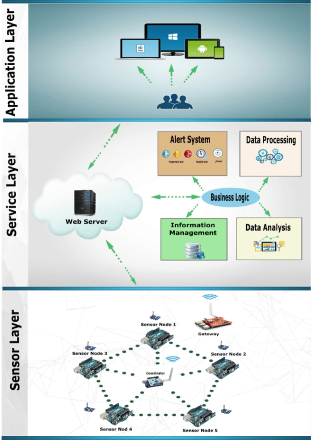
\includegraphics{Folder/images/IMG21.png}\\
    \section*{Network Protocol}
    In the context of Smart Agriculture, the IoT can be 
    described as a large set of technologies and research disciplines oriented to support the agricultural sector, through the deployment of new data-oriented system comprised of sensors, actuators, network connectivity, cloud-oriented platforms, and so on.\\
    
    Local networks, belonging to the network layer and typically including nodes equipped with sensors and/or actuators, are generally organized as Wireless Sensor Networks (WSNs). This is the general protocol which is used in IoT based smart farming.
    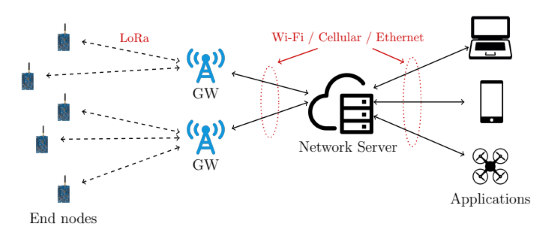
\includegraphics{Folder/images/network.png}
    %\includegraphics[scale=0.5]{Folder/net.png}//
    
    \section*{Challenges}
    The implementation and maintenance of a monitoring system in precision agriculture faces several challenges:
    
    \begin{itemize}
        \item  The greatest challenge is for sensor nodes to 
        achieve efficient and continuous operation for a long
        time in a natural environment, while taking into 
        account the climate change and wildlife interventions.
        
        \item Next Big challenge is regarding the operation of 
        a crop monitoring system with WSN and IoT technologies
        include the limited computational capabilities of 
        sensor nodes.
        
        \item Client and societal acknowledgment is another biggest problem.The reception of keen innovations will 
        without a doubt be very difficult to be easily adapted by farmers.
    \end{itemize}
    \section*{Conclusion}
    Farming can be made more efficient and accurate with the 
    implementation of IoT device. IoT can be used in different 
    domains of agriculture. Electricity and water are the main
    domains in which it can be applied.Farmers can take 
    advantage of the potential of IoT market for agriculture 
    by installing smart technologies to increase 
    competitiveness and sustainability in their productions. 
    Thus the rapid growth of population forces farmers to meet 
    the demand by implementing agricultural IoT solutions in a 
    prosperous manner.
\end{multicols}
\end{document}

